% 2010 年浙江卷理科第 21 题：椭圆 C 与直线 l 交于 A、B 两点。
% 来源 PDF：普通高考/2010/2010浙江理.pdf，SHA-256 c61b26c8cab009d567644272afc34d81e3174ffa90244c333ecfb27d61034a00。
% 原页：第 2 页（A3 三栏）第 2 栏下部，书页码 640。
% 重绘依据：椭圆中心 O，x 轴向右、y 轴向上；直线 l 与椭圆交于右上 A、左下 B，
%   直线略偏离中心、不经过 O，照原页示意。
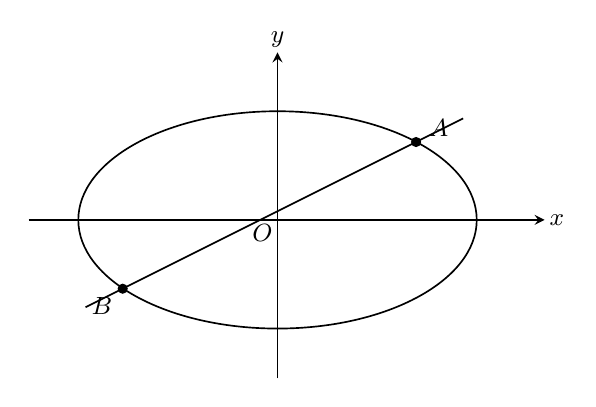
\begin{tikzpicture}[scale=1.15, semithick, every node/.style={inner sep=1.5pt, font=\small}]
  \draw (0,0) ellipse [x radius=2.2, y radius=1.2];

  % 坐标轴
  \draw[->, >=stealth] (-2.75,0) -- (2.95,0);
  \draw[->, >=stealth] (0,-1.75) -- (0,1.85);
  \node[right] at (2.95,0) {$x$};
  \node[above] at (0,1.85) {$y$};
  \node[below left] at (0,0) {$O$};

  % 直线 l 与交点
  \draw (-2.12,-0.965) -- (2.05,1.12);
  \fill (1.53,0.86) circle (1.6pt);
  \fill (-1.71,-0.76) circle (1.6pt);
  \node at (1.78,1.02) {$A$};
  \node at (-1.94,-0.95) {$B$};
\end{tikzpicture}
